\chapter{Gravity Inversion}\label{Chp:cook:gravity inversion}

\section{Introduction}

In this part of the documentation we give an introduction on how to use the
\downunder module and the inversion driver functions to perform the inversion
of gravity and magnetic data.
The driver functions enable geologists and geophysicists to apply the
\downunder module quickly and in an easy way without requiring detailed
knowledge of the theory behind inversion or programming skills.
However, users who are interested in specializing or extending the inversion
capacity are referred to Part~\ref{part2} of this manual.
It is beyond the intention of this manual to give a detailed introduction to
geophysical inversion, in particular to the appropriate preprocessing of data
sets.

The \downunder module described here is designed to calculate estimations for
the 3-D distribution of density and/or susceptibility from 2-D gravity and
magnetic data measured in ground or airborne surveys.
This process is generally called inversion of geophysical data.
Following the standard assumption it is assumed that the data are measured as
perturbation of an expected gravity and/or magnetic field of the Earth.
In this context measured gravity and magnetic data are in fact describing
anomalies in the gravity and magnetic field.
As a consequence the inversion process provides corrections to an average
density (typically $2670 kg/m^3$) and susceptibility (typically $0$).
So in the following we will always assume that given data are anomalies and
therefore not in all cases explicitly use the terms gravity anomalies or
density corrections but just use the terms gravity and density.

In this chapter we will give a detailed introduction into usage of the driver
functions for inversion of gravity data.
In the following chapters~\ref{Chp:cook:magnetic inversion} and~\ref{Chp:cook:joint inversion}
we will discuss the inversion of magnetic data, and the joint inversion of
gravity and magnetic data using \downunder.
Note, that the principles introduced in this chapter apply to magnetic and
joint inversion so the presentation for these problem classes is kept short
and users interested in magnetic data only should still work through this
chapter on gravity data. 

To run the examples discussed you need to have \escript (version 3.3.1 or
newer) installed on your computer.
Moreover, if you want to visualize the results you need to have access to a
data plotting software which is able to process \VTK input files, e.g.
\mayavi or \VisIt.
As \mayavi can be easily obtained and installed for most platforms the
tutorial includes commands to visualize output files using \mayavi .
However, it is pointed out that \VisIt is the preferred visualization tool for
\escript as it can deal with very large data sets more efficiently.
    
\begin{figure}
\centering
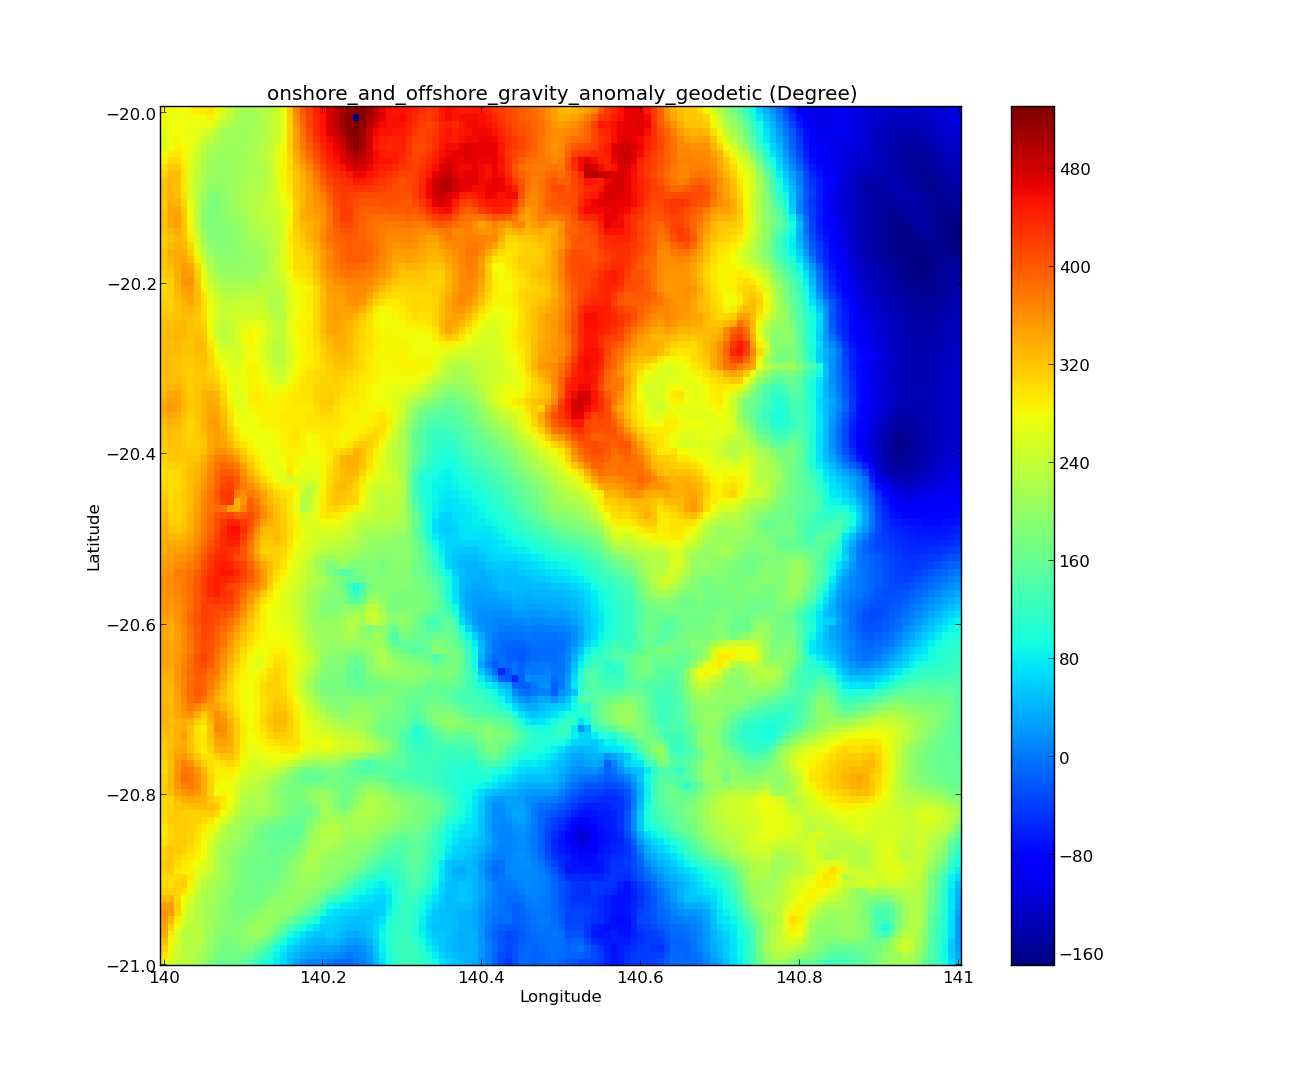
\includegraphics[width=0.7\textwidth]{QLDWestGravityDataPlot.png}
\caption{Gravity Anomaly Data in $mgal$ from Western Queensland, Australia
    (file \examplefile{data/QLDWestGravity.nc}). Data obtained from Geoscience Australia.}
%\AZADEH{Tracey R, Bacchin M, \& Wynne P. 2008. In preparation. AAGD07: A new absolute gravity datum for Australian gravity and new standards for the Australian National Gravity Database. Exploration Geophysics.}
\label{FIG:P1:GRAV:0}
\end{figure}

\begin{figure}
\centering%
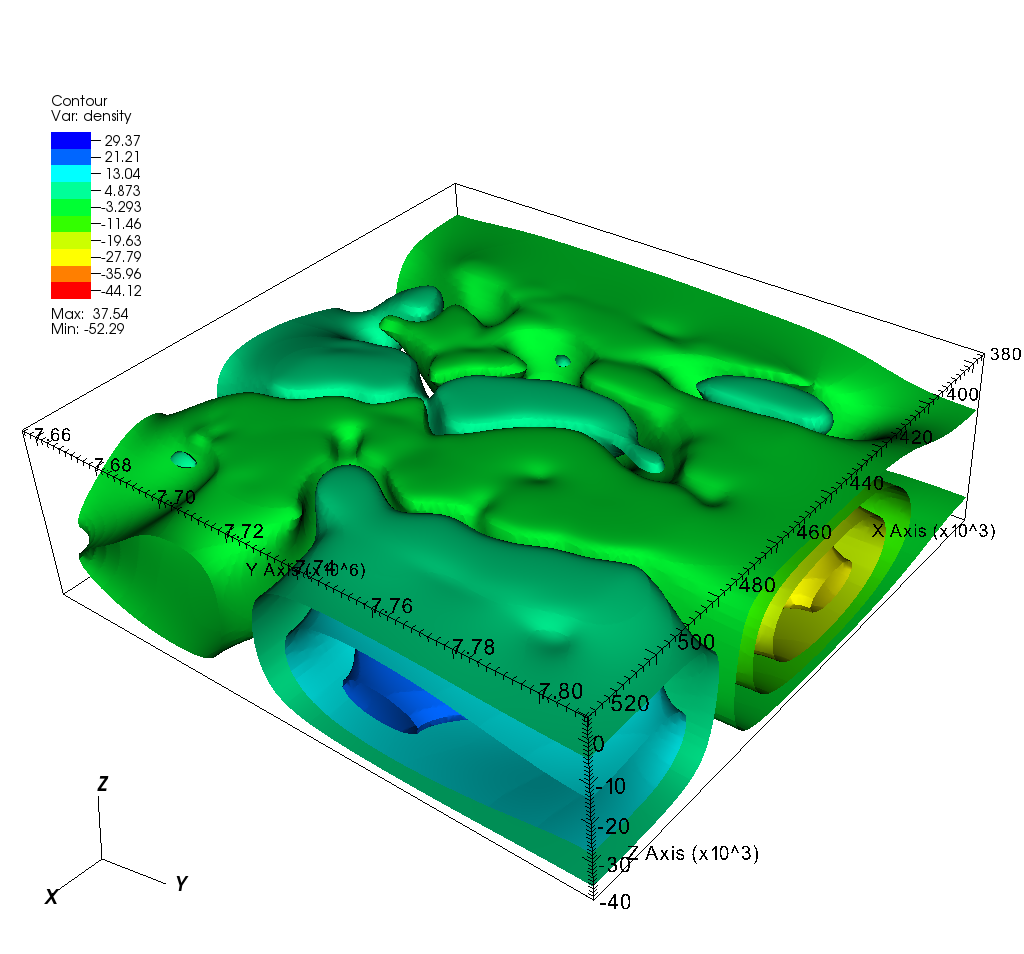
\includegraphics[width=0.9\textwidth]{QLDGravContourMu10.png}
\caption{3-D contour plot of the density distribution obtained by inversion of
    file \file{data/QLDWestGravity.nc} (with $\mu=10$).
    Colours represent values of density where high values are represented by
    blue and low values are represented by red.}
\label{FIG:P1:GRAV:1}
\end{figure}

\section{How does it work?}
The execution of the inversion is controlled by a script which, in essence, is
a text file and can be edited using any text editor.
The script contains a series of statements which are executed by an
interpreter which is an executable program reading the text file and executing
the statements line-by-line.
In the case of \downunder the interpreter is \Python.
In order to be able to process the statements in each line of the script
certain rules (called syntax) need to be obeyed.
There is a large number of online tutorials for \Python available\footnote{e.g.
\url{http://www.tutorialspoint.com/python} and \url{http://doc.pyschools.com}}.
We also refer to the \escript cook book \cite{ESCRIPTCOOKBOOK} and user's
guide \cite{ESCRIPT} which is in particular useful for users who like to dive
deeper into \downunder.
For this part of the manual no \Python knowledge is required but it is
recommended that users acquire some basic knowledge on \Python as they
progress in their work with \downunder.

The following script~\ref{code: gravity1}\footnote{The script is similar to
\examplefile{grav_netcdf.py} within the \escript example file directory.} is a
simple example to run an inversion for gravity data:

\begin{pyc}\label{code: gravity1}
\
\begin{python}
# Header:
from esys.downunder import *
from esys.weipa import *
from esys.escript import unitsSI as U

# Step 1: set up domain
dom=DomainBuilder()
dom.setVerticalExtents(depth=40.*U.km, air_layer=6.*U.km, num_cells=25)
dom.setFractionalPadding(pad_x=0.2, pad_y=0.2)
dom.fixDensityBelow(depth=40.*U.km)

# Step 2: read gravity data
source0=NetCdfData(NetCdfData.GRAVITY, 'GravitySmall.nc')
dom.addSource(source0)

# Step 3: set up inversion
inv=GravityInversion()
inv.setSolverTolerance(1e-4)
inv.setSolverMaxIterations(50)
inv.setup(dom)

# Step 4: run inversion 
inv.getCostFunction().setTradeOffFactorsModels(10.) 
rho = inv.run()

# Step 5: write reconstructed density to file
saveVTK("result.vtu", density=rho)
\end{python}
\end{pyc}
The result, in this case the density distribution, is written to an external
file for further processing. You can copy and paste the text of the script
into a file of any name, let's say for further reference we use the file
name \file{grav.py}.
It is recommended to use the extension \file{.py} to identify the file as a
\Python script.
We will discuss the statements of the script later in this chapter. 

Obviously the inversion needs to be fed with some gravity data. You can find
example data from western Queensland, Australia in two resolutions in the
\escript example directory. In this case the data are loaded from the file
\examplefile{GravitySmall.nc} which is given in the \netcdf file format.
After you have copied this file into the directory in which you have saved the
script \file{grav.py} you can run the program using the command line 
\begin{verbatim}
run-escript grav.py
\end{verbatim}
We are running \file{grav.py} through the \escript start-up command since
\escript is used as a back end for the inversion algorithm\footnote{Please see
the \escript user's guide~\cite{ESCRIPT} on how to run your script in parallel
using threading and/or MPI.}.
Obviously it is assumed that you have an installation of \escript available on
your computer, see \url{https://launchpad.net/escript-finley}.

After the execution has successfully completed you will find the result file
\file{result.vtu} in the directory from where you have started the execution
of the script.
The file has the \VTK format and can be imported easily into many
visualization tools.
One option is the \mayavi package which is available on most platforms.
You can invoke the visualization using the commands
\begin{verbatim}
mayavi2 -d result.vtu -m SurfaceMap
\end{verbatim}
from the command line.
Figure~\ref{FIG:P1:GRAV:1} shows the result of this inversion as a contour
plot\footnote{These plots were generated by \VisIt using the higher resolution
data.}, while the gravity anomaly data is shown in Figure~\ref{FIG:P1:GRAV:0}.
We will discuss data later in Section~\ref{SEC:P1:GRAV:DATA}.

Let us take a closer look at the script\footnote{In \Python lines starting
with `\#` are comments and are not processed further.}. Besides the header
section one can separate the script into five steps:
\begin{enumerate}
    \item set up domain on which the inversion problem is solved
    \item load the data 
    \item set-up the inversion problem
    \item run the inversion
    \item further processing of the result. Here we write the reconstructed
          density distribution to a file.
\end{enumerate}
In the following we will discuss the steps of the scripts in more detail.
Before we do this it is pointed out that the header section, following
\Python conventions, makes all required packages available to access within
the script.
At this point we will not discuss this in more details but emphasize that the
header section is a vital part of the script.
It is is required in each \downunder inversion script and should not be
altered except if additional modules are needed.

\begin{figure}
\centering
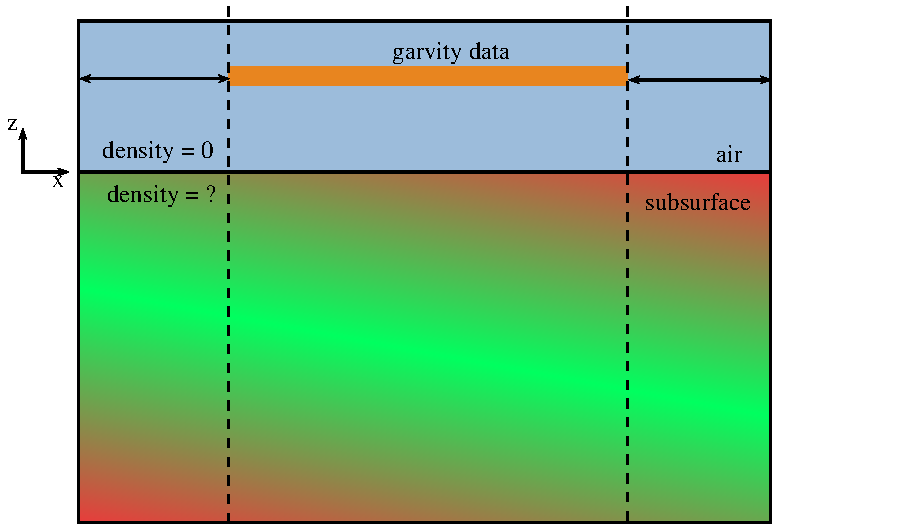
\includegraphics[width=\textwidth]{dom2D.pdf}
\caption{2-D domain set-up for gravity inversion}
\label{FIG:P1:GRAV:2}
\end{figure}

\section{Creating the Inversion Domain}
First step in Script~\ref{code: gravity1} is the definition of the domain over
which the inversion is performed.
We think of the domain as a block with orthogonal, plain faces.
Figure~\ref{FIG:P1:GRAV:2} shows the set-up for a two-dimensional domain
(see also Figure~\ref{fig:domainBuilder} for 3-D).
The lateral coordinates along the surface of the Earth are denoted by $x$ and
$y$ (only $x$-direction is used in 2-D).
The $z$ direction defines the vertical direction where the part above the
surface has positive coordinates and the subsurface negative coordinates.
The height of the section above the surface, which is assumed to be filled
with air, needs to be set by the user.
The inversion assumes that the density in the section is known to be
zero\footnote{Always keeping in mind that these are not absolute values but
anomalies.}.
The density below the surface is unknown and is calculated through the
inversion. The user needs to specify the depth below the surface in which the
density is to be calculated.
The lateral extension of the domain is defined by the data sets fed into the
inversion.
It is chosen large enough to cover all data sets (in case more than one is
used). In order to reduce the impact of the boundary a padding zone around the
data sets can be introduced.

\begin{figure}
\centering
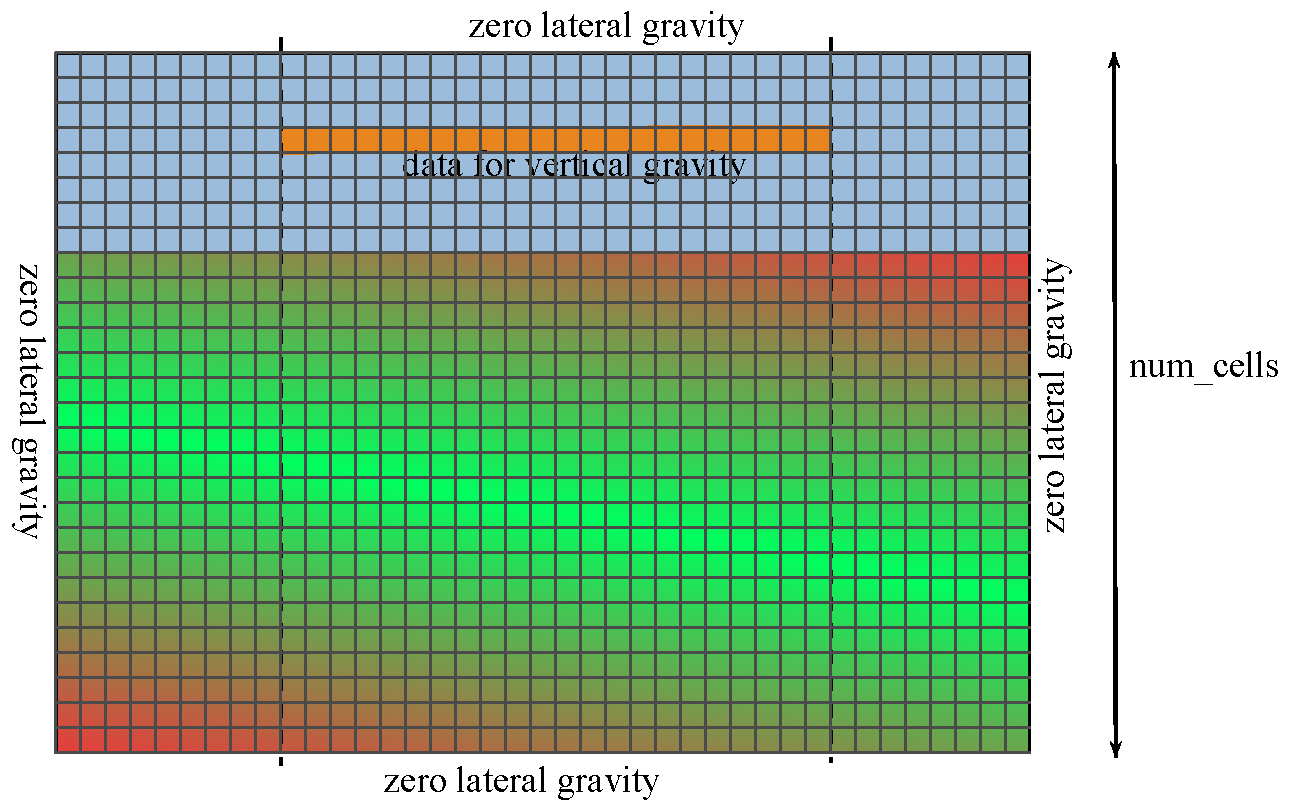
\includegraphics[width=\textwidth]{dom2DFEM.pdf}
\caption{Cell distribution and boundary conditions for a 2-D domain}
\label{FIG:P1:GRAV:3}
\end{figure}

The reconstruction of the gravity field from an estimated density distribution
is the key component of the inversion process.
To do this \downunder uses the finite element method (FEM).
We need to introduce a grid over the domain, see Figure~\ref{FIG:P1:GRAV:3}.
The number of vertical cells is set by the user while the number of horizontal
cells is derived from the grid spacing of the gravity data set(s).
It is assumed that gravity field data given are constant across a cell.
To be able to reconstruct the gravity field some assumptions on the values of
the gravity field on the domain boundary have to be made.
\downunder assumes that on all faces the lateral gravity field component
equals zero. No assumptions on the horizontal components are
made\footnote{It is assumed that the gravity potential equals zero on the top
and bottom surface, see Section~\ref{sec:forward gravity} for details}%
\footnote{Most inversion codes use Green's functions over an unbounded domain
to reconstruct the gravity field. This approach makes the assumption that the
gravity field (or potential) is converging to zero when moving away from the
region of interest. The boundary conditions used here are stronger in the
sense that the lateral gravity component is enforced to be zero in a defined
distance of the region of interest but weaker in the sense that no constraint
on the horizontal component is applied.}.
   
In script~\ref{code: gravity1} the statement
\begin{verbatim}
dom=DomainBuilder()
\end{verbatim}
creates something like a factory to build a domain.
We then define the features of the domain we would like to create:
\begin{verbatim}
dom.setVerticalExtents(depth=40.*U.km, air_layer=6.*U.km, num_cells=25)
dom.setFractionalPadding(pad_x=0.2, pad_y=0.2)
\end{verbatim}
Here we specify the depth of the domain to $40 km$, the thickness of the air
layer above the surface to $6 km$ and the number of vertical cells to $25$.
We also introduce a lateral padding of $20 \%$ of the expansion of the gravity
data on each side of the data and in both lateral directions.

In some cases it can be appropriate to assume that the density below a certain
depth is zero\footnote{As we are in fact calculating density corrections this
means that the density is assumed to be the average density.}.
The statement 
\begin{verbatim}
dom.fixDensityBelow(depth=40.*U.km)
\end{verbatim}
introduces this constraint.
As in the case discussed here if the depth for zero density is not less than
the depth of the domain no constraint at depth is applied to the density.

\downunder uses the metre-kilogram-second based International System of Units
(SI)\footnote{see \url{http://en.wikipedia.org/wiki/International_System_of_Units}}\index{SI}.
So all values must be converted to appropriate units.
This does not apply to geographic coordinates which in \downunder are given in
fractional degrees (as a floating point number) to represent longitude and
latitude. In the script we have used the expression
\begin{verbatim}
depth=40.*U.km
\end{verbatim}
to define the depth of the domain to $40 km$.
The expression \verb|U.km| denotes the unit $km$ (kilometer) and ensures
appropriate conversion of the value $40$ into the base unit $m$ (meter).
It is recommended to add units to values (where present) in order to make sure
that the final values handed into \downunder is given with the appropriate
units.
The physical units module of \escript, which we have imported here under the
name \verb|U| in the script header, defines a large number of physical units
and constants, please see~\cite{ESCRIPT} and~\cite{ESCRIPTONLINE}. 

\section{Loading Gravitational Data}\label{SEC:P1:GRAV:DATA}
In practice gravity acceleration is measured in various ways, for instance by
airborne surveys~\cite{Telford1990a}.
\downunder assumes that all data supplied as input are already appropriately
pre-processed. In particular, corrections for
\begin{itemize}
 \item free-air, to remove effects from altitude above ground;
 \item latitude, to remove effects from ellipsoidicity of the Earth;
 \item terrain, to remove effects from topography
\end{itemize}
must have been applied to the data.
In general, data prepared in such a form are called Bouguer anomalies~\cite{Telford1990a}.

To load gravity data into \downunder the data are given on a plane parallel
to the surface of the Earth at a constant altitude, see
diagram~\ref{FIG:P1:GRAV:2}.
The data need to be defined over a rectangular grid covering a subregion of
the Earth surface.
The grid uses a geographic coordinate system with latitudes and longitudes
assumed to be given in the Clarke 1866 geodetic system.
Figure~\ref{FIG:P1:GRAV:0} shows an example of such a data set from the
western parts of Queensland, Australia.
The data set covers a rectangular region between $140^o$ and $141^o$ east
and between $20^o$ and $21^o$ south.
Notice that latitude varies between $-90^o$ to $90^o$ where negative signs
refer to places in the southern hemisphere and longitude varies between
$-180^o$ to $180^o$ where negative signs refer to places west of Greenwich.
The colour at a location represents the value of the vertical Bouguer gravity
anomaly at this point at the surface of the Earth.
Values in this data set range from $-160 \; mgal$ to about $500 \; mgal$\footnote{The unit
$mgal$ means milli $gal$ (galileo) with $1 \; gal = 0.01 \frac{m}{sec^2}$.}
over a $121 \times 121$ grid.

In general, a patch of gravity data needs to be defined over a plane
\verb|NX| $\times$ \verb|NY| where \verb|NX| and \verb|NY| define the number
of grid lines in the longitude (\verb|X|) and the latitude (\verb|Y|)
direction, respectively.
The grid is spanned from an origin with spacing \verb|DELTA_X| and
\verb|DELTA_Y| in the longitude and the latitude direction, respectively.
The gravity data for all grid points need to be given as an \verb|NX|
$\times$ \verb|NY| array.
If available, measurement errors can be associated with the gravity data.
The values are given as an \verb|NX| $\times$ \verb|NY| array matching the
shape of the gravity array.
Note that data need not be available on every single point of the grid, see
Section~\ref{SEC:P1:GRAV:REMARK:DATAHOLES} for more information on this.

Currently, two data file formats are supported, namely \emph{ER Mapper Raster}
\cite{ERMAPPER} files and \netcdf~\cite{NETCDF} files.
In the examples of this chapter we use \netcdf files and refer to
Section~\ref{SEC:P1:GRAV:REMARK:ERMAPPER} and
Section~\ref{sec:ref:DataSource:ERM} for more information on using ER Mapper
Raster files.
If you have data in any other format you have the option of writing a suitable
reader (for advanced users, see Chapter~\ref{Chp:ref:data sources}) or,
assuming you are able to read the data in \Python, refer to the example
script \examplefile{create_netcdf.py} which shows how to create a file
in the \netcdf file format~\cite{NETCDF} compatible with \downunder from
a data array.

In script~\ref{code: gravity1} we use the statement 
\begin{verbatim}
source0=NetCdfData(NetCdfData.GRAVITY, 'GravitySmall.nc')
\end{verbatim}
to load the gravity data stored in \examplefile{GravitySmall.nc} in the
\netcdf format. 
Within the script the data set is now available under the name \verb|source0|.
We need to link the data set to the \verb|DomainBuilder| using 
\begin{verbatim}
dom.addSource(source0)
\end{verbatim}
At the time the domain for the inversion is built the \verb|DomainBuilder|
will use the information about origin, extent and spacing along with the other
options provided to build an appropriate domain.
As at this point a flat Earth is assumed geographic coordinates used to
represent data in the input file are mapped to a (local) Cartesian coordinate
system. This is achieved by projecting the geographic coordinates into the
\emph{Universal Transverse Mercator} (UTM) coordinate system\footnote{See e.g.
\url{http://en.wikipedia.org/wiki/Universal_Transverse_Mercator_coordinate_system}}.

There are a few optional arguments you can add when constructing a data source.
While Section~\ref{sec:ref:DataSource} has a detailed description of all
arguments it is worth noting a few.
Firstly, it is important to know that data slices are assumed to be at altitude
$0$ by default. This can be easily changed though:
\begin{verbatim}
source0=NetCdfData(NetCdfData.GRAVITY, 'GravitySmall.nc', altitude=2.5*U.km)
\end{verbatim}
Another important setting is the scale or unit of the measurements.
The default is dependent on the data type and for gravity anomalies a scale
of $\frac{\mu m}{sec^2}$ (or $0.1 \; mgal$) is assumed. For instance to 
change the default scale to $mgal$ (which is $10^{-5} \frac{m}{sec^2}$),
you could use:
\begin{verbatim}
source0=NetCdfData(NetCdfData.GRAVITY, 'GravitySmall.nc', scale_factor=U.mgal)
\end{verbatim}
Finally, it is possible to specify measurement errors (i.e. uncertainties)
alongside the data.
Since these can never be zero, a value of $2$ units is used if nothing else
has been specified.
The error value is assumed to be given in the same units as the data so the
default value translates to an error of $0.2 \; mgal$.
There are two possibilities to specify the error, namely by providing a
constant value which is applied to all data points:
\begin{verbatim}
source0=NetCdfData(NetCdfData.GRAVITY, 'GravitySmall.nc', error=1.7)
\end{verbatim}
or, if the information is available in the same \netcdf file under the name
\verb|errors|, provide \downunder with the appropriate variable name:
\begin{verbatim}
source0=NetCdfData(NetCdfData.GRAVITY, 'GravitySmall.nc', error="errors")
\end{verbatim}


It is important to keep an eye on the complexity of the inversion.
A good measure is the total number of cells being used.
Assume we have given a data set on a $20 \times 20$ grid and we add lateral
padding of, say, $20 \%$ to each side of the data, the lateral number of cells
becomes $(20\cdot 1.4)\times (20\cdot 1.4)=1.4^2\cdot 20^2\approx 2\cdot 10^2=800$.
If we use $20$ cells in the vertical direction we end up with a total number
of $800 \times 20 = 16,000$ cells.
This size can be easily handled by a modern desktop PC.
If we increase the grid size of the data to $40 \times 40$ points and use $40$
cells in the vertical extent we get a total of $(2\cdot 40^2)\cdot 40=128,000$
cells, a problem size which is considerably larger but can still be handled by
a desktop computer.
Taking this one step further, if the amount of data is increased to
$200\times 200$ points and we use $200$ cells in the vertical extent the
domain will contain $16,000,000$ ($16$ million) cells.
This scenario requires a computer with enough memory and (a) fast processor(s)
to run the inversion.
This estimate of complexity growth applies to the case where the increase
of data grid size is driven by an increase of resolution where it is
recommended to increase the vertical resolution in synch with the lateral
resolution. Note that if more than one data set is used the target resolution
will be the resolution of the finest data set (see also
Section~\ref{SEC:P1:GRAV:REMARK:MULTIDATA}).
In other cases the expansion of the region of interest drives an increase of
data grid size and the increase of total number of cells is less dramatic as
the vertical number of cells can remain constant while keeping a balanced
resolution in vertical and lateral direction.

\section{Setting up the Inversion and Running it}
We are now at step three of script~\ref{code: gravity1} in which the actual
inversion is set up.
First we create an empty inversion under the name \verb|inv|:
\begin{verbatim}
inv=GravityInversion()
\end{verbatim}
As indicated by the name we can use \verb|inv| to perform an inversion of
gravity data\footnote{\verb|GravityInversion| is a driver with a simplified
interface which is provided for convenience. See Part~\ref{part2} for more
details on how to write inversion scripts with more general functionality, e.g.
constraints.}. The inversion is an iterative process which sequentially
calculates updates to the density distribution in an attempt to improve the
match of the gravity field produced by the density distribution with the data.
Termination of the iteration is controlled by the tolerance which is set by
the user:
\begin{verbatim}
inv.setSolverTolerance(1e-4)
\end{verbatim}
Here we set the tolerance to $10^{-4}$, i.e. the iteration is terminated if
the maximum density correction is less than or equal to $10^{-4}$ relative to
the maximum value of estimated density anomaly.
In case the iteration does not converge a maximum number of iteration steps is
set:
\begin{verbatim}
inv.setSolverMaxIterations(50)
\end{verbatim}
If the maximum number of iteration steps (here $50$) is reached the iteration
process is aborted and an error message is printed.
In this case you can try to rerun the inversion with a larger value for the
maximum number of iteration steps.
If even for a very large number of iteration steps no convergence is achieved,
it is very likely that the inversion has not been set up properly.

The statement 
\begin{verbatim}
inv.setup(dom)
\end{verbatim}
links the inversion with the domain and the data.
At this step -- as we are solving a gravity inversion problem -- only
gravitational data attached to the domain builder \verb|dom| are considered.
Internally a cost function $J$ is created which is minimized during the
inversion iteration.
It is a combination of a measure of the data misfit of the gravity field from
the given density distribution and a measure of the smoothness of the density
distribution.
The latter is often called the regularization term.
By default the gradient of density is used as the regularization term, see
also Section~\ref{SEC:P1:GRAV:REMARK:REG}.
Obviously, the result of the inversion is sensitive to the weighting between
the misfit and the regularization.
This trade-off factor $\mu$ for the misfit function is set by the following
statement:
\begin{verbatim}
inv.getCostFunction().setTradeOffFactorsModels(0.1) 
\end{verbatim}
Here we set $\mu=0.1$. The statement \verb|inv.setup| must appear in the
script before setting the trade-off factor.
A small value for the trade-off factor $\mu$ will give more emphasis to the
regularization component and create a smoother density distribution.
A large value of the trade-off factor $\mu$ will emphasize the misfit more
and typically creates a better fit to the data and a rougher density
distribution.
It is important to keep in mind that the regularization reduces noise in the
date and in fact gives the problem a unique solution.
Consequently, the trade-off factor $\mu$ may not be chosen too large in order
control the noise on the solution and ensure convergence in the iteration
process.

We can now actually run the inversion:
\begin{verbatim}
rho = inv.run()
\end{verbatim}
The answer as calculated during the inversion is returned and can be accessed
under the name \verb|rho|.
As pointed out earlier the iteration process may fail in which case the
execution of the script is aborted with an error message.

\section{Taking a Look}
In the final step of script~\ref{code: gravity1} the calculated density
distribution is written to an external file.
A popular file format used by several visualization packages such as
\VisIt~\cite{VISIT} and \mayavi~\cite{mayavi} is the \VTK file format.
The result of the inversion which has been named \verb|rho| can be written to
the file \file{result.vtu} by adding the statement
\begin{verbatim}
saveVTK("result.vtu", density=rho)
\end{verbatim}
at the end of script.
The inversion solution is tagged with the name \verb|density| in the result
file, however any other name for the tag could be used.
As the format is text-based (as opposed to binary) \VTK files tend to be very
large and take compute time to create, in particular when it comes to large
numbers of cells ($>10^6$).
For large problems it is more efficient to use the \SILO file format~\cite{SILO}.
\SILO files tend to be smaller and are faster generated and read.
It is the preferred format to import results into the visualization program
\VisIt~\cite{VISIT} which is particularly suited for the visualization of
large data sets.
Inversion results can directly exported into \SILO files using the statement
\begin{verbatim}
saveSilo("result.silo", density=rho)
\end{verbatim}
replacing the \verb|saveVTK(...)| statement.
Similar to \VTK files the result \verb|rho| is tagged with the name
\verb|density| so it can be identified in the visualization program.

Another useful output option is the \Voxet format which is understood by the
\GOCAD\cite{GOCAD} geologic modelling software.
In order to write inversion results to \Voxet files use the statement
\begin{verbatim}
saveVoxet("result.vo", density=rho)
\end{verbatim}
Unlike the other output formats \Voxet data consists of a header file with the
file extension \verb|.vo| and separate \emph{property} files without file
extension. The call to \verb|saveVoxet(...)| above would produce the files
\file{result.vo} and \file{result_density}.

\begin{figure}
    \begin{center}
        \subfigure[$\mu=0.1$]{%
            \label{FIG:P1:GRAV:10 MU01}
            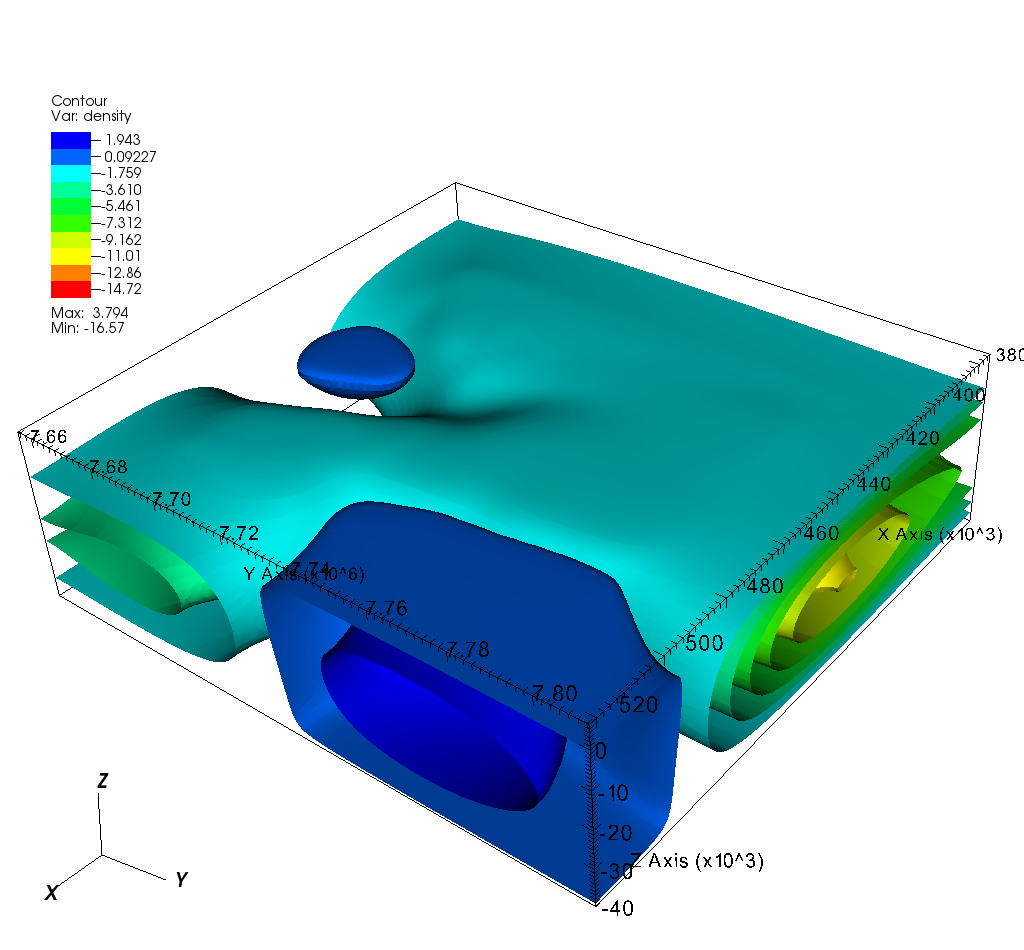
\includegraphics[width=0.45\textwidth]{QLDGravContourMu01.png}
        }%
        \subfigure[$\mu=1.$]{%
            \label{FIG:P1:GRAV:10 MU1}
            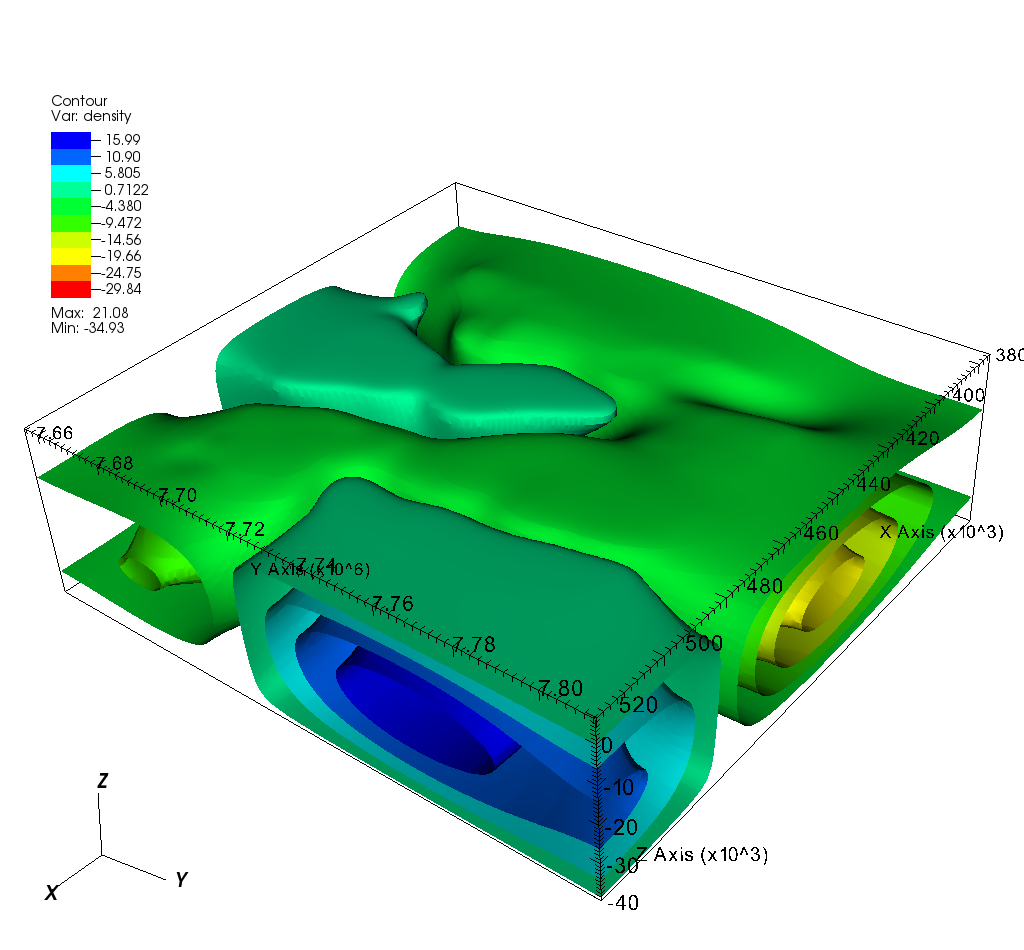
\includegraphics[width=0.45\textwidth]{QLDGravContourMu1.png}
        }\\ %  ------- End of the first row ----------------------%
        \subfigure[$\mu=10.$]{%
            \label{FIG:P1:GRAV:10 MU10}
            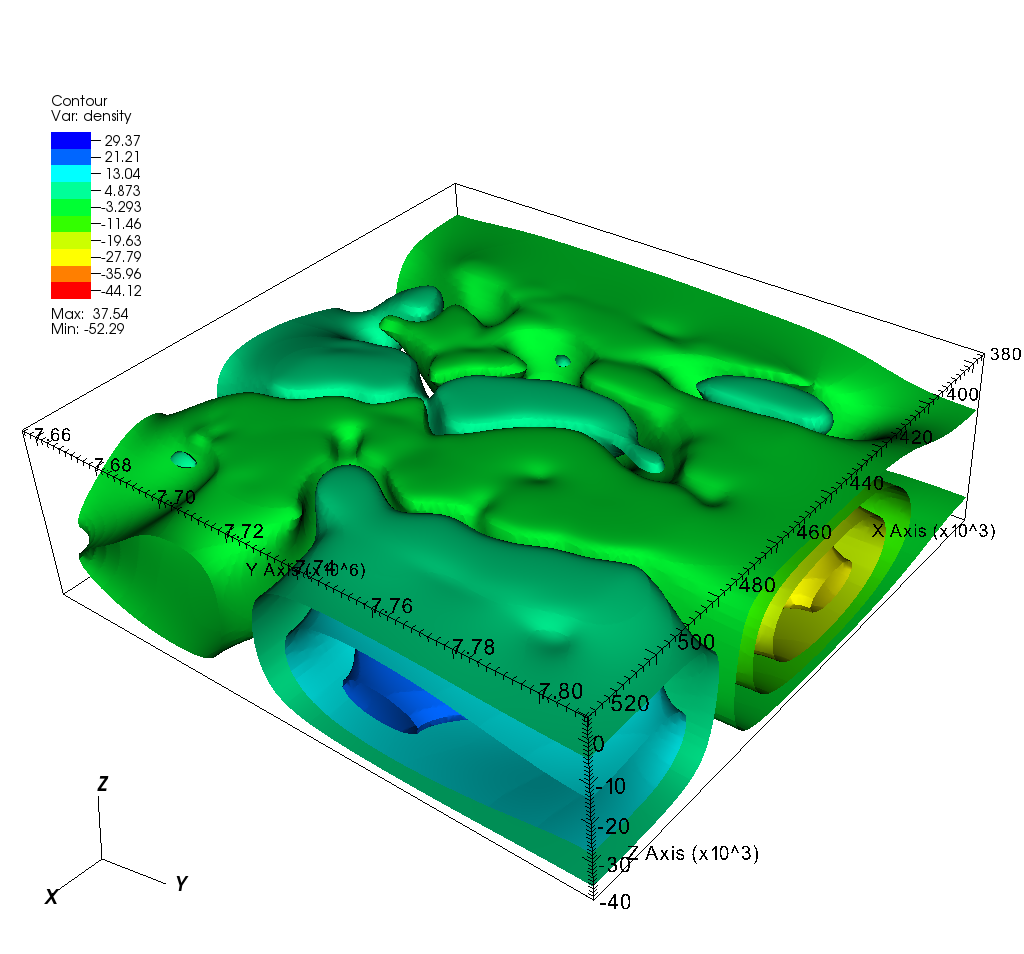
\includegraphics[width=0.45\textwidth]{QLDGravContourMu10.png}
        }%
        \subfigure[$\mu=100.$]{%
            \label{FIG:P1:GRAV:10 MU100}
            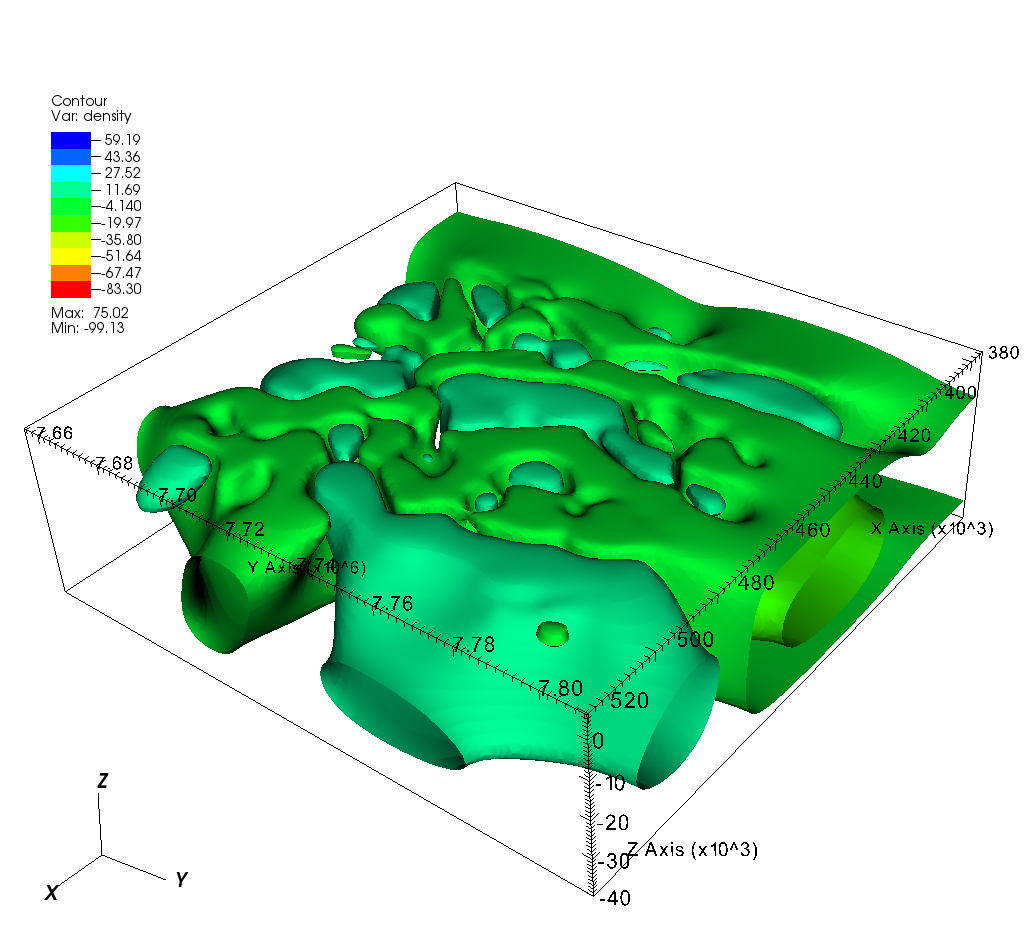
\includegraphics[width=0.45\textwidth]{QLDGravContourMu100.png}
        }\\ %  ------- End of the second row ----------------------%
        \subfigure[$\mu=1000.$]{%
            \label{FIG:P1:GRAV:10 MU1000}
            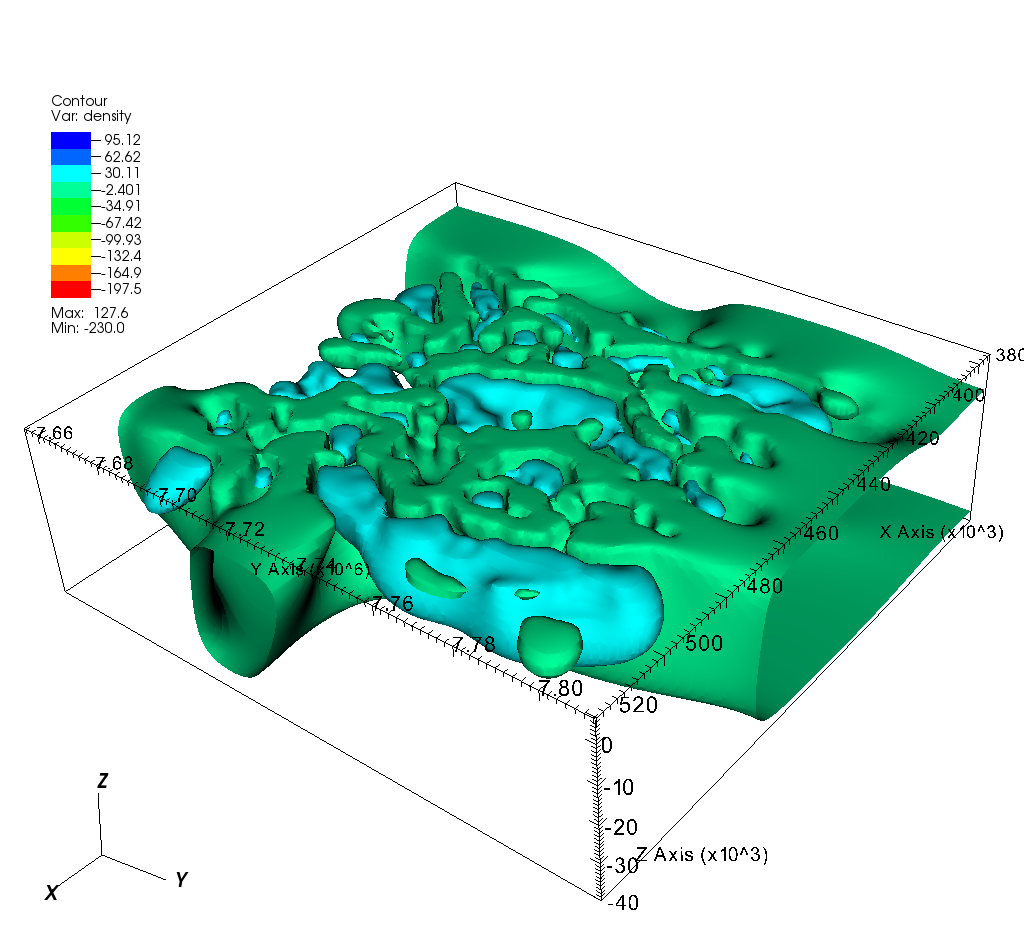
\includegraphics[width=0.45\textwidth]{QLDGravContourMu1000.png}
        }%
    \end{center}
    \caption{3-D contour plots of gravity inversion results with data from
    Figure~\ref{FIG:P1:GRAV:0} for various values of the model trade-off
    factor $\mu$. Visualization has been performed in \VisIt.}
    \label{FIG:P1:GRAV:10}
\end{figure}

\begin{figure}
    \begin{center}
        \subfigure[$\mu=0.1$]{%
            \label{FIG:P1:GRAV:11 MU01}
            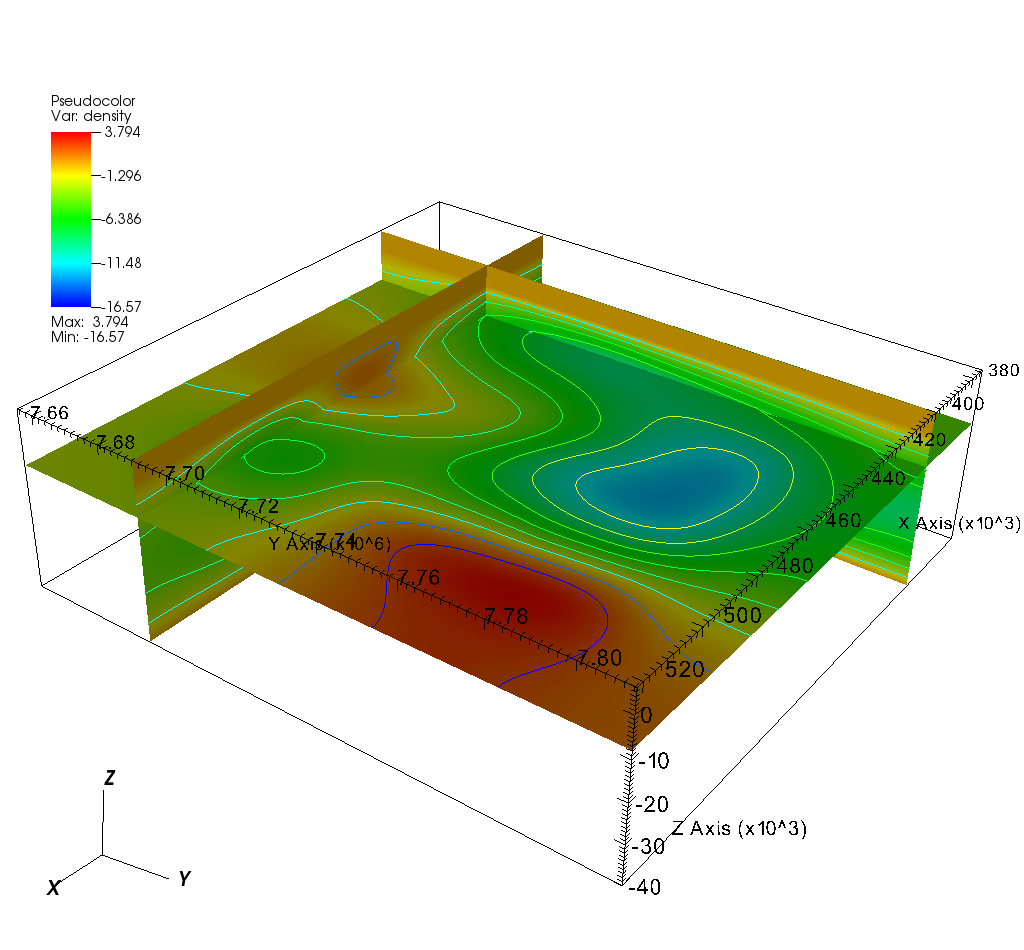
\includegraphics[width=0.45\textwidth]{QLDGravDepthMu01.png}
        }%
        \subfigure[$\mu=1.$]{%
            \label{FIG:P1:GRAV:11 MU1}
            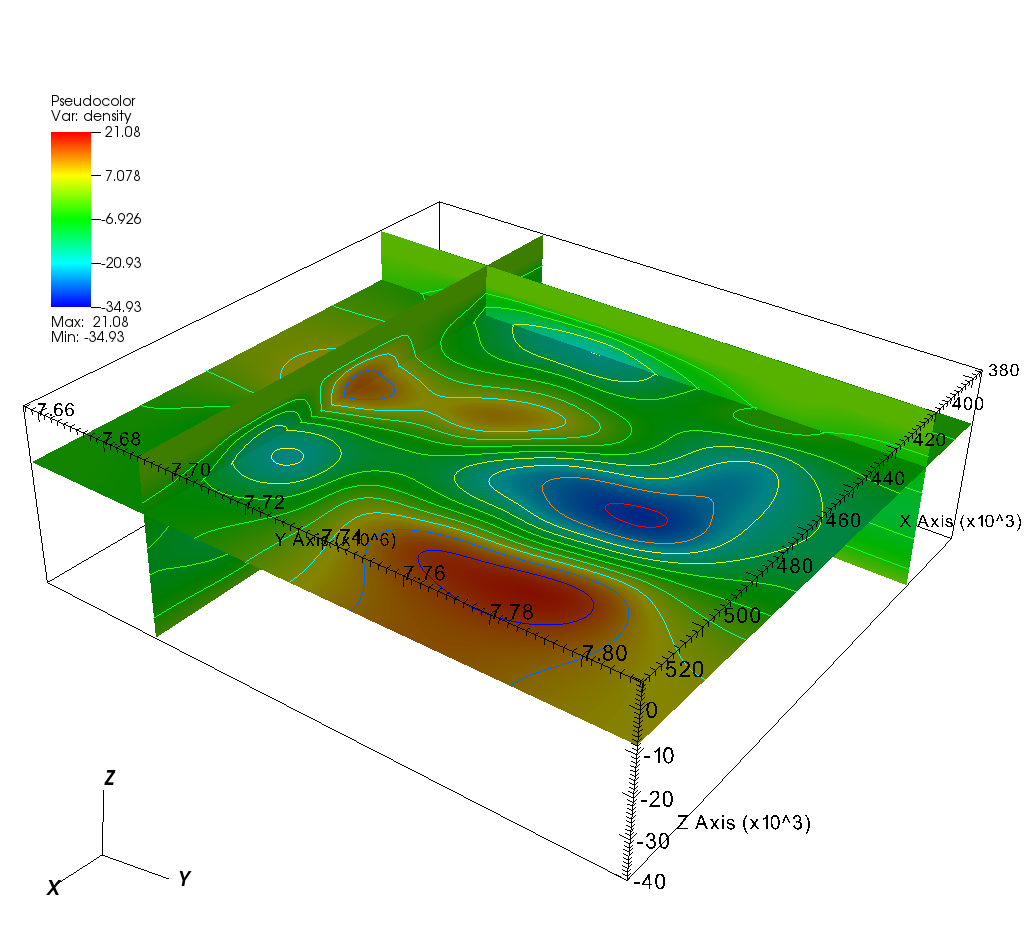
\includegraphics[width=0.45\textwidth]{QLDGravDepthMu1.png}
        }\\ %  ------- End of the first row ----------------------%
        \subfigure[$\mu=10.$]{%
            \label{FIG:P1:GRAV:11 MU10}
            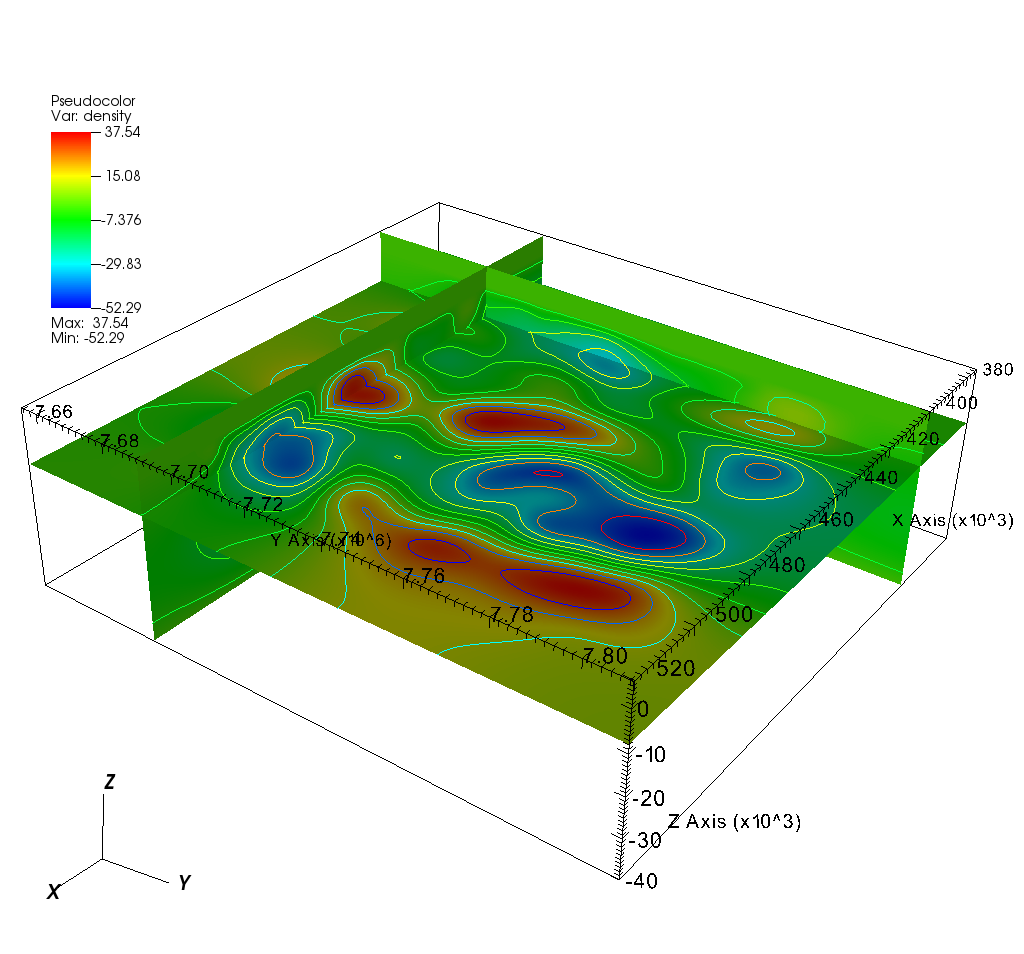
\includegraphics[width=0.45\textwidth]{QLDGravDepthMu10.png}
        }%
        \subfigure[$\mu=100.$]{%
            \label{FIG:P1:GRAV:11 MU100}
            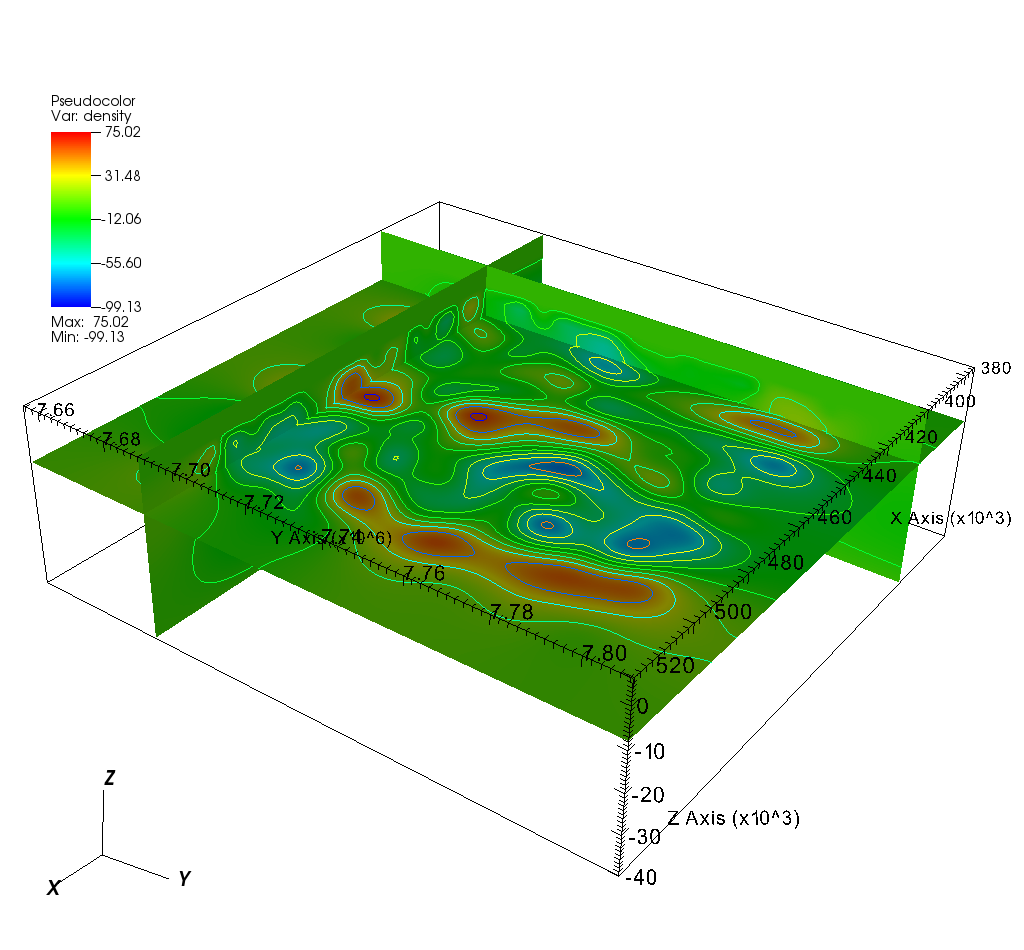
\includegraphics[width=0.45\textwidth]{QLDGravDepthMu100.png}
        }\\ %  ------- End of the second row ----------------------%
        \subfigure[$\mu=1000.$]{%
            \label{FIG:P1:GRAV:11 MU1000}
            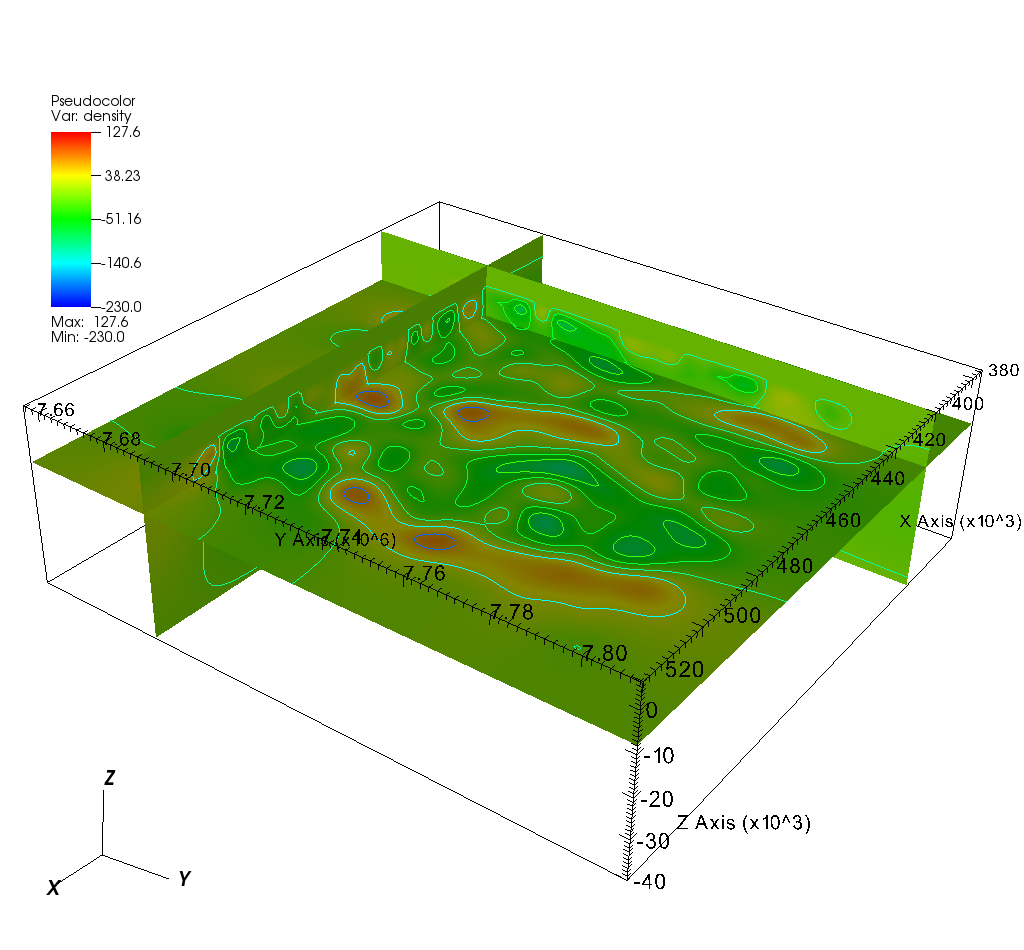
\includegraphics[width=0.45\textwidth]{QLDGravDepthMu1000.png}
        }%
    \end{center}
    \caption{3-D slice plots of gravity inversion results with data from
    Figure~\ref{FIG:P1:GRAV:0} for various values of the model trade-off
    factor $\mu$. Visualization has been performed \VisIt.%
    }
%    \AZADEH{check images.}
    \label{FIG:P1:GRAV:11}
\end{figure}

Figures~\ref{FIG:P1:GRAV:10} and~\ref{FIG:P1:GRAV:11} show two different
styles of visualization generated in \VisIt using the result of the inversion
of the gravity anomalies shown in Figure~\ref{FIG:P1:GRAV:0}.
The inversions have been performed with different values for the model
trade-off factor $\mu$.
The visualization shows clearly the smoothing effect of lower values for the
trade-off factors.
For larger values of the trade-off factor the density distribution becomes
rougher showing larger details.
Computational costs are significantly higher for larger trade-off factors.
Moreover, noise in the data has a higher impact on the result.
Typically several runs are required to adjust the value for the trade-off
factor to the datasets used.

For some analysis tools it is useful to process the results in form of
Comma-separated Values (\CSV)\footnote{see 
\url{http://en.wikipedia.org/wiki/Comma-separated_values}}.
Such a file can be created using the statement
\begin{verbatim}
saveDataCSV("result.csv", x=rho.getFunctionSpace().getX(), density=rho)
\end{verbatim}
in the script.
This will create a \file{result.csv} with columns separated by a comma.
Each row contains the value of the density distribution and the three
coordinates of the corresponding location in the domain.
There is a header specifying the meaning of the corresponding column.
Notice that rows are not written in a particular order and therefore, if
necessary, the user has to apply appropriate sorting of the rows.
Columns are written in alphabetic order of their corresponding tag names.
For the interested reader: the statement \verb|rho.getFunctionSpace()| returns
the type used to store the density data \verb|rho|.
The \verb|getX()| method returns the coordinates of the sampling points used
for the particular type of representation, see~\cite{ESCRIPT} for details. 

\section{Remarks}

\subsection{ER Mapper Raster Files}\label{SEC:P1:GRAV:REMARK:ERMAPPER}
The \downunder module can read data stored in ER Mapper Raster files. A data
set in this format consists of two files, a header file whose name usually ends
in \verb|.ers| and the actual data file which has the same filename as the
header file but without any file extension.
These files are usually produced by a commercial software package and the
contents can be quite diverse.
Therefore, it is not guaranteed that every data set is supported by \downunder
but the most common types of raster data should work\footnote{If your data
does not load please contact us through \url{https://launchpad.net/escript-finley}.}.

The interface for loading ER Mapper files is very similar to the \netcdf
interface described in Section~\ref{SEC:P1:GRAV:DATA}.
To load gravity data stored in the file pair\footnote{These files are available
in the example directory.} \examplefile{GravitySmall.ers} (the
header) and \examplefile{GravitySmall} (the data) without changing any of the
defaults use:
\begin{verbatim}
source0=ErMapperData(ErMapperData.GRAVITY, 'GravitySmall.ers')
\end{verbatim}
If your data set does not follow the default naming convention you can specify
the name of the data file explicitly:
\begin{verbatim}
source0=ErMapperData(ErMapperData.GRAVITY, 'GravitySmall.ers',
                     datafile='GravityData')
\end{verbatim}
Please note that there is no way for the reader to determine if the two files
really form a pair so make sure to pass the correct filenames when constructing
the reader object.
The same optional arguments explained in sections \ref{SEC:P1:GRAV:DATA} and
\ref{SEC:P1:GRAV:REMARK:DATAHOLES} are available for ER Mapper data sets.
However, due to the limitation of the file format only a constant error value
is supported.

\subsection{Data With Holes}\label{SEC:P1:GRAV:REMARK:DATAHOLES}
As described previously in this chapter input data is always given in the form
of a rectangular grid with constant cell size in each dimension.
However, there are cases when this is not necessarily the case.
Consider an onshore data set which includes parts of the offshore region as in
Figure~\ref{FIG:P1:GRAV:onshoreoffshore}.
The valid data in this example has a value range of about $-600$ to $600$ and
the inversion is to be run based on these values only, disregarding the
offshore region.
In order to achieve that, the offshore region is \emph{masked} by using a
constant value which is not found within the onshore area.
Figure~\ref{FIG:P1:GRAV:onshoreoffshore} clearly shows this masked area in
dark blue since a mask value of $-1000$ was used.

\begin{figure}[ht]
    \centering
    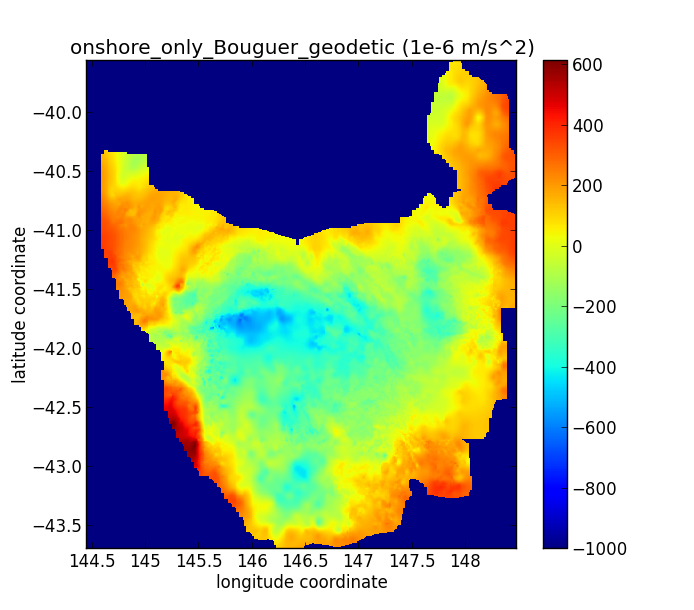
\includegraphics[width=0.45\textwidth]{onshore-offshore.png}
    \caption{Plot of a rectangular gridded onshore data set that includes
    offshore regions which have a value (here $-1000$) not found within the
    real data (Bouguer anomalies in Tasmania, courtesy Geoscience Australia)}
    \label{FIG:P1:GRAV:onshoreoffshore}
\end{figure}

The \netcdf conventions supported in \downunder include a standard way of
specifying such a mask value.
The example script \examplefile{create_netcdf.py} demonstrates how this is
accomplished in an easy way with any data.
If, for any reason, the mask value in the input file is invalid it can be
overridden via the \verb|null_value| argument when constructing the
\verb|NetCdfData| object:
\begin{verbatim}
source0=NetCdfData(NetCdfData.GRAVITY, 'data0.nc', null_value=-1000)
\end{verbatim}
In this example, all data points that have a value of $-1000$ are ignored and
not used in the inversion.
Please note that the special value \emph{NaN} (not-a-number) is sometimes used
for the purposes of masking in data sets.
Areas marked with this value are always disregarded in \downunder.

\subsection{Multiple Data Sets}\label{SEC:P1:GRAV:REMARK:MULTIDATA}
It is possible to run a single inversion using more than one input data set,
possibly in different file formats.
To do so, simply create the data sources and add them to the domain builder:
\begin{verbatim}
source0=NetCdfData(NetCdfData.GRAVITY, 'data0.nc')
source1=ErMapperData(ErMapperData.GRAVITY, 'data1.ers')
dom.addSource(source0)
dom.addSource(source1)
\end{verbatim}
However, there are some restrictions when combining data sets:
\begin{itemize}
    \item Due to the coordinate transformation all data sets must be located in
        the same UTM zone. If a single dataset crosses UTM zones only the zone
        of the central longitude is used when projecting.
        For example, if one data set lies mostly in zone 51 but contains areas
        of zone 52, it is transformed using zone 51. In this case more data
        from zone 51 can be added, but not from any other zone.
    \item All data sets should have the same spatial resolution but this is not
        enforced. Combining data with different resolution is currently
        considered experimental but works best when the resolutions are
        multiples of each other. For example if the first data set has a
        resolution (or cell size) of $100$ metres and the second has a cell
        size of $50$ metres then the target domain will have a cell size of
        $50$ metres (the finer resolution) and each point of the coarse data
        will occupy two cells (in the respective dimension).
\end{itemize}

\subsection{Regularization Term}\label{SEC:P1:GRAV:REMARK:REG}
The \verb|GravityInversion| class supports the following form for the
regularization:
\begin{equation}
\int w^{(0)} \cdot \rho^2 + w^{(1)}_0  \rho_{,0}^2 +  w^{(1)}_1  \rho_{,1}^2 +  w^{(1)}_2  \rho_{,2}^2\; dx   
\end{equation}
where the integral is calculated across the entire domain.
$\rho$ represents the density distribution where $\rho_{,0}$ $\rho_{,1}$ and
$\rho_{,2}$ are the spatial derivatives of $\rho$ with respect to the two
lateral and the vertical direction, respectively.
$w^{(0)}$, $w^{(1)}_0$, $w^{(1)}_1$ and $w^{(1)}_2$ are weighting
factors\footnote{A more general form, e.g. spatially variable values for the
weighting factors, is supported, see Part~\ref{part2}}.
By default these are $w^{(0)}=0$, $w^{(1)}_0=w^{(1)}_1=w^{(1)}_2=1$.
Other weighting factors can be set in the inversion set-up.
For instance to set $w^{(0)}=10$, $w^{(1)}_0=w^{(1)}_1=0$ and $w^{(1)}_2=100$
use the statement:
\begin{verbatim}
inv.setup(dom, w0=10, w1=[0,0,100])
\end{verbatim}
It is pointed out that the weighting factors are rescaled in order to improve
numerical stability. Therefore the relative size of the weighting factors is
relevant and using
\begin{verbatim}
inv.setup(dom, w0=0.1, w1=[0,0,1])
\end{verbatim}
would lead to the same regularization as the statement above.
